\addcontentsline{toc}{section}{\textbf{ANEXOS}}

\begin{landscape}
\begin{table}[htbp]
\centering
\scriptsize
\caption{Anexo 1: Matriz de Consistencia de la Investigación - Ecosistema SynapTome}
\label{tab:matriz_consistencia_synaptome}

\renewcommand{\arraystretch}{1.3}
\setlength{\tabcolsep}{3pt}

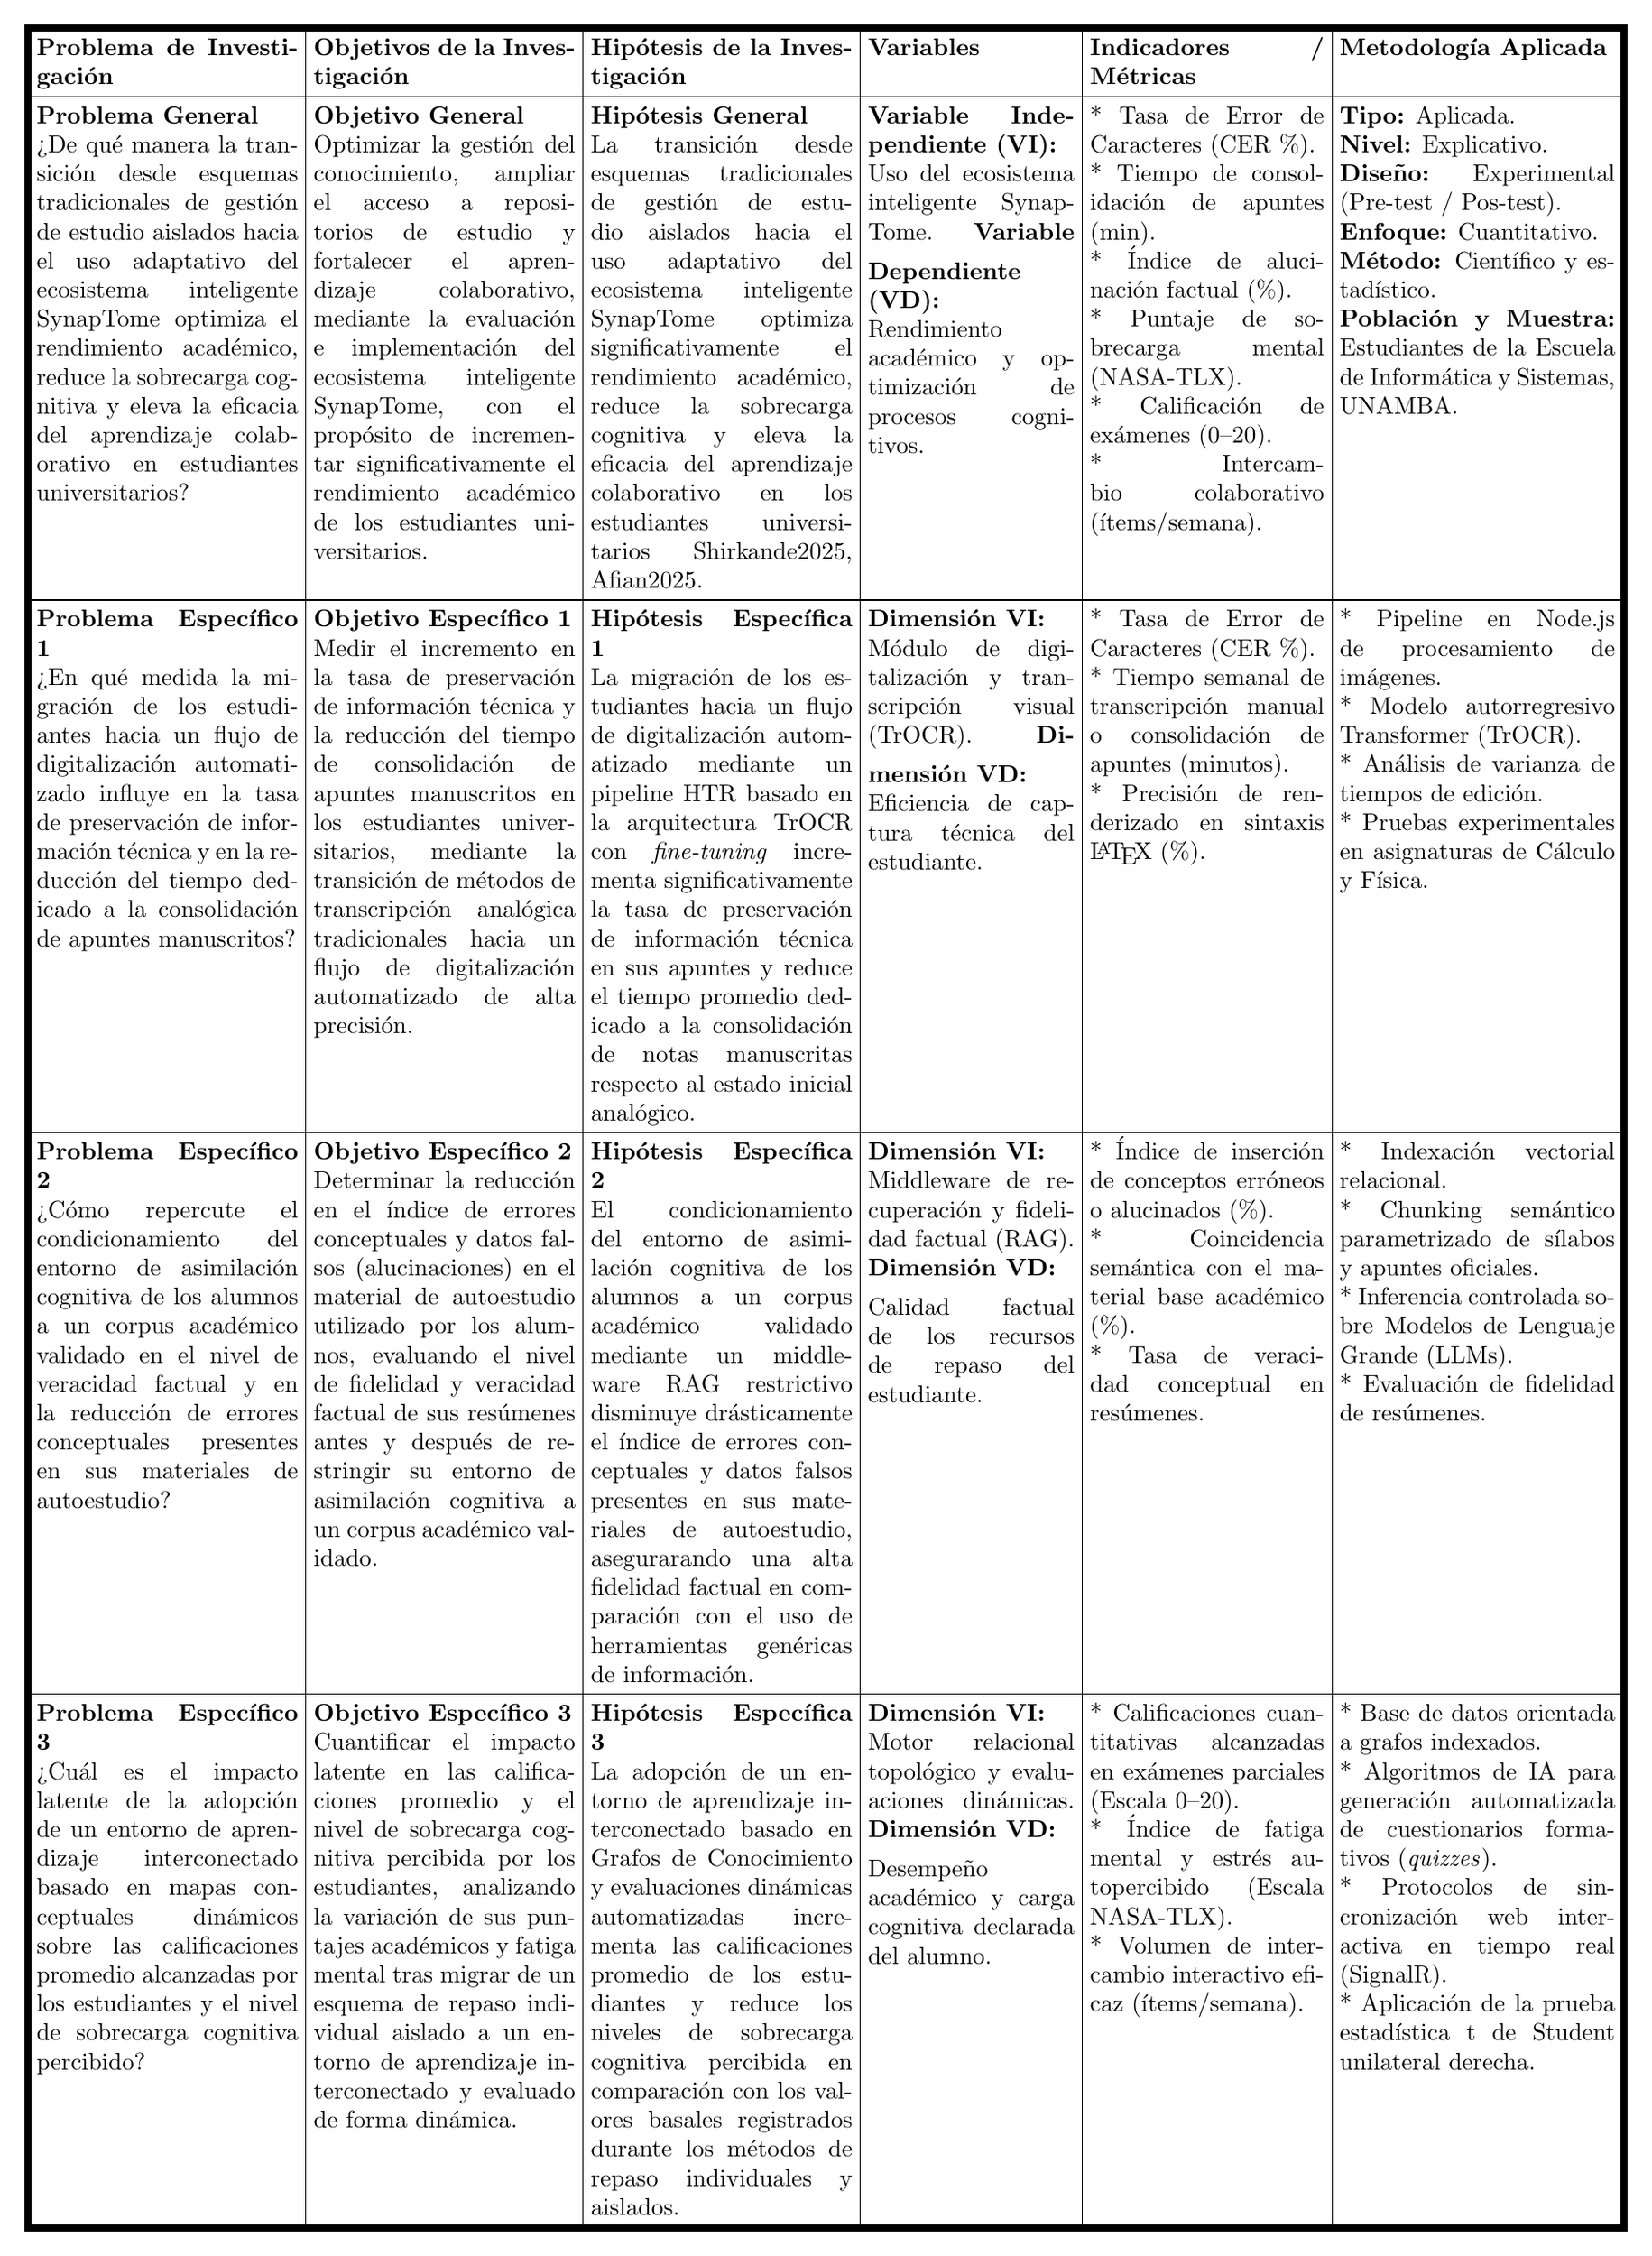
\begin{tikzpicture}
\node[inner sep=0pt] (tabla) {
\begin{tabular}{|p{3.8cm}|p{3.8cm}|p{3.8cm}|p{3.0cm}|p{3.4cm}|p{4.0cm}|}
\hline
\textbf{Problema de Investigación} &
\textbf{Objetivos de la Investigación} &
\textbf{Hipótesis de la Investigación} &
\textbf{Variables} &
\textbf{Indicadores / Métricas} &
\textbf{Metodología Aplicada} \\
\hline
\thickhline

%====================================================
% NIVEL GENERAL
%====================================================
\textbf{Problema General} \newline
¿De qué manera la transición desde esquemas tradicionales de gestión de estudio aislados hacia el uso adaptativo del ecosistema inteligente SynapTome optimiza el rendimiento académico, reduce la sobrecarga cognitiva y eleva la eficacia del aprendizaje colaborativo en estudiantes universitarios? &

\textbf{Objetivo General} \newline
Optimizar la gestión del conocimiento, ampliar el acceso a repositorios de estudio y fortalecer el aprendizaje colaborativo, mediante la evaluación e implementación del ecosistema inteligente SynapTome, con el propósito de incrementar significativamente el rendimiento académico de los estudiantes universitarios. &

\textbf{Hipótesis General} \newline
La transición desde esquemas tradicionales de gestión de estudio aislados hacia el uso adaptativo del ecosistema inteligente SynapTome optimiza significativamente el rendimiento académico, reduce la sobrecarga cognitiva y eleva la eficacia del aprendizaje colaborativo en los estudiantes universitarios \parencite{Shirkande2025, Afian2025}. &

\textbf{Variable Independiente (VI):} \newline
Uso del ecosistema inteligente SynapTome.
\vspace{0.15cm}
\textbf{Variable Dependiente (VD):} \newline
Rendimiento académico y optimización de procesos cognitivos. &

* Tasa de Error de Caracteres (CER \%). \newline
* Tiempo de consolidación de apuntes (min). \newline
* Índice de alucinación factual (\%). \newline
* Puntaje de sobrecarga mental (NASA-TLX). \newline
* Calificación de exámenes (0--20). \newline
* Intercambio colaborativo (ítems/semana). &

\textbf{Tipo:} Aplicada. \newline
\textbf{Nivel:} Explicativo. \newline
\textbf{Diseño:} Experimental (Pre-test / Pos-test). \newline
\textbf{Enfoque:} Cuantitativo. \newline
\textbf{Método:} Científico y estadístico. \newline
\textbf{Población y Muestra:} Estudiantes de la Escuela de Informática y Sistemas, UNAMBA. \\
\hline

%====================================================
% ESPECIFICO 1
%====================================================
\textbf{Problema Específico 1} \newline
¿En qué medida la migración de los estudiantes hacia un flujo de digitalización automatizado influye en la tasa de preservación de información técnica y en la reducción del tiempo dedicado a la consolidación de apuntes manuscritos? &

\textbf{Objetivo Específico 1} \newline
Medir el incremento en la tasa de preservación de información técnica y la reducción del tiempo de consolidación de apuntes manuscritos en los estudiantes universitarios, mediante la transición de métodos de transcripción analógica tradicionales hacia un flujo de digitalización automatizado de alta precisión. &

\textbf{Hipótesis Específica 1} \newline
La migración de los estudiantes hacia un flujo de digitalización automatizado mediante un pipeline HTR basado en la arquitectura TrOCR con \textit{fine-tuning} incrementa significativamente la tasa de preservación de información técnica en sus apuntes y reduce el tiempo promedio dedicado a la consolidación de notas manuscritas respecto al estado inicial analógico. &

\textbf{Dimensión VI:} \newline
Módulo de digitalización y transcripción visual (TrOCR).
\vspace{0.15cm}
\textbf{Dimensión VD:} \newline
Eficiencia de captura técnica del estudiante. &

* Tasa de Error de Caracteres (CER \%). \newline
* Tiempo semanal de transcripción manual o consolidación de apuntes (minutos). \newline
* Precisión de renderizado en sintaxis \LaTeX{} (\%). &

* Pipeline en Node.js de procesamiento de imágenes. \newline
* Modelo autorregresivo Transformer (TrOCR). \newline
* Análisis de varianza de tiempos de edición. \newline
* Pruebas experimentales en asignaturas de Cálculo y Física. \\
\hline

%====================================================
% ESPECIFICO 2
%====================================================
\textbf{Problema Específico 2} \newline
¿Cómo repercute el condicionamiento del entorno de asimilación cognitiva de los alumnos a un corpus académico validado en el nivel de veracidad factual y en la reducción de errores conceptuales presentes en sus materiales de autoestudio? &

\textbf{Objetivo Específico 2} \newline
Determinar la reducción en el índice de errores conceptuales y datos falsos (alucinaciones) en el material de autoestudio utilizado por los alumnos, evaluando el nivel de fidelidad y veracidad factual de sus resúmenes antes y después de restringir su entorno de asimilación cognitiva a un corpus académico validado. &

\textbf{Hipótesis Específica 2} \newline
El condicionamiento del entorno de asimilación cognitiva de los alumnos a un corpus académico validado mediante un middleware RAG restrictivo disminuye drásticamente el índice de errores conceptuales y datos falsos presentes en sus materiales de autoestudio, asegurarando una alta fidelidad factual en comparación con el uso de herramientas genéricas de información. &

\textbf{Dimensión VI:} \newline
Middleware de recuperación y fidelidad factual (RAG).
\vspace{0.15cm}
\textbf{Dimensión VD:} \newline
Calidad factual de los recursos de repaso del estudiante. &

* Índice de inserción de conceptos erróneos o alucinados (\%). \newline
* Coincidencia semántica con el material base académico (\%). \newline
* Tasa de veracidad conceptual en resúmenes. &

* Indexación vectorial relacional. \newline
* Chunking semántico parametrizado de sílabos y apuntes oficiales. \newline
* Inferencia controlada sobre Modelos de Lenguaje Grande (LLMs). \newline
* Evaluación de fidelidad de resúmenes. \\
\hline

%====================================================
% ESPECIFICO 3
%====================================================
\textbf{Problema Específico 3} \newline
¿Cuál es el impacto latente de la adopción de un entorno de aprendizaje interconectado basado en mapas conceptuales dinámicos sobre las calificaciones promedio alcanzadas por los estudiantes y el nivel de sobrecarga cognitiva percibido? &

\textbf{Objetivo Específico 3} \newline
Cuantificar el impacto latente en las calificaciones promedio y el nivel de sobrecarga cognitiva percibida por los estudiantes, analizando la variación de sus puntajes académicos y fatiga mental tras migrar de un esquema de repaso individual aislado a un entorno de aprendizaje interconectado y evaluado de forma dinámica. &

\textbf{Hipótesis Específica 3} \newline
La adopción de un entorno de aprendizaje interconectado basado en Grafos de Conocimiento y evaluaciones dinámicas automatizadas incrementa las calificaciones promedio de los estudiantes y reduce los niveles de sobrecarga cognitiva percibida en comparación con los valores basales registrados durante los métodos de repaso individuales y aislados. &

\textbf{Dimensión VI:} \newline
Motor relacional topológico y evaluaciones dinámicas.
\vspace{0.15cm}
\textbf{Dimensión VD:} \newline
Desempeño académico y carga cognitiva declarada del alumno. &

* Calificaciones cuantitativas alcanzadas en exámenes parciales (Escala 0--20). \newline
* Índice de fatiga mental y estrés autopercibido (Escala NASA-TLX). \newline
* Volumen de intercambio interactivo eficaz (ítems/semana). &

* Base de datos orientada a grafos indexados. \newline
* Algoritmos de IA para generación automatizada de cuestionarios formativos (\textit{quizzes}). \newline
* Protocolos de sincronización web interactiva en tiempo real (SignalR). \newline
* Aplicación de la prueba estadística t de Student unilateral derecha. \\
\hline

\end{tabular}
};

\draw[line width=3pt] (tabla.north west) rectangle (tabla.south east);
\end{tikzpicture}
\end{table}
\end{landscape}